\documentclass[a4paper]{ltjsarticle}

\usepackage[dvipdfmx]{graphicx}
\usepackage[dvipdfmx,hidelinks,pdfusetitle]{hyperref}
\hypersetup{
    colorlinks=false,
    bookmarksnumbered=true,
    pdfborder={0 0 0},
    bookmarkstype=toc
}
\usepackage[nobreak]{cite}
\usepackage{pxjahyper}
\usepackage{amsmath}
\usepackage{tikz}

\usetikzlibrary{datavisualization}
\usetikzlibrary{positioning}
\usetikzlibrary{shapes.geometric, shapes.misc}
\usetikzlibrary{patterns}
\usetikzlibrary{calc}

\begin{document}

% ====================

\begin{itembox}[l]{東京工業大学 1997年}
    $a^{2}x^{2}+b^{2}y^{2}\leqq 1$ を満たす $(x,\ y)$ がすべて $a(x-1)+b(y-1)\leqq 0$ を満たすような $(a,\ b)$ の範囲を求め,図示せよ.
\end{itembox}

$X=ax$, $Y=by$ とおくと,$a^{2}x^{2}+b^{2}y^{2}\leqq 0$ より,

\begin{equation}
    X^2+Y^2\leqq 1\label{eq:1}
\end{equation}

また,$a(x-1)+b(y-1)\leqq 0$ より

\begin{equation}
    X+Y\leqq a+b\label{eq:2}
\end{equation}

となる.

\begin{enumerate}[label=(\roman*)]
    \item $a\neq 0$ かつ $b\neq 0$ のとき

          \begin{equation*}
              \text{「\eqref{eq:1}を満たす}(X,\ Y)\text{がすべて\eqref{eq:2}を満たす」とは,「円\eqref{eq:1}が半円面\eqref{eq:2}に含まれる」}\tag{\ast}
          \end{equation*}

          ことと同値である.よって,$a,\ b$ の満たすべき条件は,$\sqrt{2}\leqq a+b$ となる.

    \item $a\neq 0$ かつ $b=0$ のとき

          $Y=0$ により ($\ast$) は「 $X^2\leqq 1$ を満たす $X$ がすべて $X\leqq a$ を満たす」ことで,$a$ の満たすべき条件は $a\geqq 1$ となる.

    \item $a=0$ かつ $b\neq 0$ のとき

          (ii)と同様にして $b\geqq 1$ となる.

    \item $a=0$ かつ $b=0$ のとき

          $X=Y=0$ であるから\eqref{eq:2}式は常に成り立つ.
\end{enumerate}

以上から,点 $(a,\ b)$ の存在範囲は下図の網目部分(境界を含む),太線部分および●の点となる。

\begin{figure}[!ht]
    \centering
    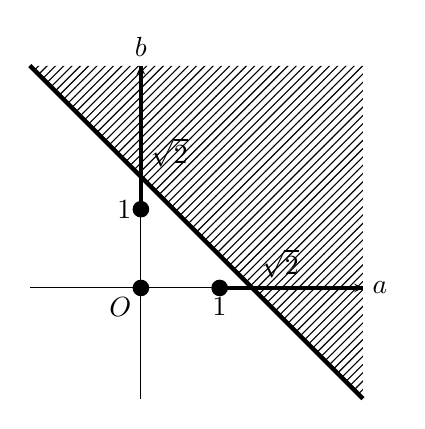
\begin{tikzpicture}
        \draw[domain=-1.41:2.82, smooth, variable=\x, ultra thick] plot ({\x},{sqrt(2)-\x});
        \fill[gray!80, pattern=north east lines] (-1.41,2.82) -- (2.82,2.82) -- (2.82,-1.41) -- cycle;
        \node[above right] at (0, 1.41) {$\sqrt{2}$};
        \node[above right] at (1.41, 0) {$\sqrt{2}$};
        \draw[ultra thick] (1,0) -- (2.82,0);
        \draw[ultra thick] (0,1) -- (0,2.82);
        \fill (0,0) circle (3pt);
        \fill (1,0) circle (3pt);
        \fill (0,1) circle (3pt);
        \node[left] at (0, 1) {$1$};
        \node[below] at (1, 0) {$1$};

        \draw[->,>=stealth] (-1.41,0) -- (2.82,0) node[right] {$a$};
        \draw[->,>=stealth] (0,-1.41) -- (0,2.82) node[above] {$b$};
        \node[below left] at (0,0) {$O$};
    \end{tikzpicture}
\end{figure}

% ====================

\end{document}
